% This template has been tested with IEEEtran of 2015.

% !TeX spellcheck = en-US
% !TeX encoding = utf8
% !TeX program = pdflatex
% !BIB program = bibtex
% -*- coding:utf-8 mod:LaTeX -*-

%cmap has to be loaded before any font package (such as newtxmath)
\RequirePackage{cmap}

% DO NOT DOWNLOAD IEEEtran.cls - Use the one of your LaTeX distribution
\documentclass[conference]{IEEEtran}[2015/08/26]

% Balance the last page
% The pbalance package (see https://ctan.org/pkg/pbalance) "just works" (in contrast to balance.sty or other solutions)
\usepackage{balance}

% use nicer font for code
\usepackage[zerostyle=b,scaled=.75]{newtxtt}

% for demonstration purposes
\usepackage{mwe}

\usepackage[T1]{fontenc}
\usepackage[utf8]{inputenc} %support umlauts in the input

\usepackage{graphicx}

%Set English as language and allow to write hyphenated"=words
\usepackage[ngerman,main=english]{babel}
%Hint by http://tex.stackexchange.com/a/321066/9075 -> enable "= as dashes
\addto\extrasenglish{\languageshorthands{ngerman}\useshorthands{"}}

% backticks (`) are rendered as such in verbatim environment. See https://tex.stackexchange.com/a/341057/9075 for details.
\usepackage{upquote}

%extended enumerate, such as \begin{compactenum}
\usepackage{paralist}

%for easy quotations: \enquote{text}
\usepackage{csquotes}

%enable margin kerning
\RequirePackage{iftex}
\ifPDFTeX
  \RequirePackage[%
    final,%
    expansion=alltext,%
    protrusion=alltext-nott]{microtype}%
\else
  \RequirePackage[%
    final,%
    protrusion=alltext-nott]{microtype}%
\fi%
% \texttt{test -- test} keeps the "--" as "--" (and does not convert it to an en dash)
\DisableLigatures{encoding = T1, family = tt* }

%tweak \url{...}
\usepackage{url}
%\urlstyle{same}
%improve wrapping of URLs - hint by http://tex.stackexchange.com/a/10419/9075
\makeatletter
\g@addto@macro{\UrlBreaks}{\UrlOrds}
\makeatother
%nicer // - solution by http://tex.stackexchange.com/a/98470/9075
%DO NOT ACTIVATE -> prevents line breaks
%\makeatletter
%\def\Url@twoslashes{\mathchar`\/\@ifnextchar/{\kern-.2em}{}}
%\g@addto@macro\UrlSpecials{\do\/{\Url@twoslashes}}
%\makeatother

% Diagonal lines in a table - http://tex.stackexchange.com/questions/17745/diagonal-lines-in-table-cell
% Slashbox is not available in texlive (due to licensing) and also gives bad results. This, we use diagbox
%\usepackage{diagbox}

\usepackage{booktabs}

% Required for package pdfcomment later
\usepackage{xcolor}

% For listings
\usepackage{listings}
\lstset{%
  basicstyle=\ttfamily,%
  columns=fixed,%
  basewidth=.5em,%
  xleftmargin=0.5cm,%
  captionpos=b}%

% Enable nice comments
\usepackage{pdfcomment}
%
\newcommand{\commentontext}[2]{\colorbox{yellow!60}{#1}\pdfcomment[color={0.234 0.867 0.211},hoffset=-6pt,voffset=10pt,opacity=0.5]{#2}}
\newcommand{\commentatside}[1]{\pdfcomment[color={0.045 0.278 0.643},icon=Note]{#1}}
%
% Compatibility with packages todo, easy-todo, todonotes
\newcommand{\todo}[1]{\commentatside{#1}}
% Compatiblity with package fixmetodonotes
\newcommand{\TODO}[1]{\commentatside{#1}}

% Bibliopgraphy enhancements
%  - enable \cite[prenote][]{ref}
%  - enable \cite{ref1,ref2}
% Alternative: \usepackage{cite}, which enables \cite{ref1, ref2} only (otherwise: Error message: "White space in argument")
%
% Doc: http://texdoc.net/natbib
\ifCLASSOPTIONcompsoc
  % IEEE Computer Society needs nocompress option at cite.sty
  % natbib includes the same functionality
  \usepackage[%
    square,        % for square brackets
    comma,         % use commas as separators
    numbers,       % for numerical citations;
    sort           % orders multiple citations into the sequence in which they appear in the list of references;
    %sort&compress % as sort but in addition multiple numerical citations
                   % are compressed if possible (as 3-6, 15);
  ]{natbib}
\else
  % normal IEEE
  \usepackage[%
    square,        % for square brackets
    comma,         % use commas as separators
    numbers,       % for numerical citations;
    %sort           % orders multiple citations into the sequence in which they appear in the list of references;
    sort&compress % as sort but in addition multiple numerical citations
                   % are compressed if possible (as 3-6, 15);
  ]{natbib}
\fi
% Same fontsize as without natbib
\renewcommand{\bibfont}{\normalfont\footnotesize}
% Enable hyperlinked author names in the case of \citet
% Source: https://tex.stackexchange.com/a/76075/9075
\usepackage{etoolbox}
\makeatletter
\patchcmd{\NAT@test}{\else \NAT@nm}{\else \NAT@hyper@{\NAT@nm}}{}{}
\makeatother

% Enable that parameters of \cref{}, \ref{}, \cite{}, ... are linked so that a reader can click on the number an jump to the target in the document
\usepackage{hyperref}
% Enable hyperref without colors and without bookmarks
\hypersetup{hidelinks,
  colorlinks=true,
  allcolors=black,
  pdfstartview=Fit,
  breaklinks=true}
%
% Enable correct jumping to figures when referencing
\usepackage[all]{hypcap}

%enable \cref{...} and \Cref{...} instead of \ref: Type of reference included in the link
\usepackage[capitalise,nameinlink]{cleveref}
\crefname{lstlisting}{\lstlistingname}{\lstlistingname}
\Crefname{lstlisting}{Listing}{Listings}

%Following definitions are outside of IfPackageLoaded; inside, they are not visible
%
%Intermediate solution for hyperlinked refs. See https://tex.stackexchange.com/q/132420/9075 for more information.
\newcommand{\Vlabel}[1]{\label[line]{#1}\hypertarget{#1}{}}
\newcommand{\lref}[1]{\hyperlink{#1}{\FancyVerbLineautorefname~\ref*{#1}}}

\newenvironment{listing}[1][htbp!]{\begin{figure}[#1]}{\end{figure}}
\newcounter{listing}

\usepackage{xspace}
%\newcommand{\eg}{e.\,g.\xspace}
%\newcommand{\ie}{i.\,e.\xspace}
\newcommand{\eg}{e.\,g.,\ }
\newcommand{\ie}{i.\,e.,\ }

%introduce \powerset - hint by http://matheplanet.com/matheplanet/nuke/html/viewtopic.php?topic=136492&post_id=997377
\DeclareFontFamily{U}{MnSymbolC}{}
\DeclareSymbolFont{MnSyC}{U}{MnSymbolC}{m}{n}
\DeclareFontShape{U}{MnSymbolC}{m}{n}{
  <-6>    MnSymbolC5
  <6-7>   MnSymbolC6
  <7-8>   MnSymbolC7
  <8-9>   MnSymbolC8
  <9-10>  MnSymbolC9
  <10-12> MnSymbolC10
  <12->   MnSymbolC12%
}{}
\DeclareMathSymbol{\powerset}{\mathord}{MnSyC}{180}

% *** SUBFIGURE PACKAGES ***
\ifCLASSOPTIONcompsoc
  \usepackage[caption=false,font=footnotesize,labelfont=sf,textfont=sf]{subfig}
\else
  \usepackage[caption=false,font=footnotesize]{subfig}
\fi

\usepackage{stfloats}

% correct bad hyphenation here
\hyphenation{op-tical net-works semi-conduc-tor}






\begin{document}
%\IEEEoverridecommandlockouts

\title{Quick start for LaTeXing with IEEEtran.cls for\\ IEEE Conferences}

\author{%
  \IEEEauthorblockN{Oliver Kopp}
  \IEEEauthorblockA{University of Stuttgart, Germany\\
    \{lastname\}@ipvs.uni-stuttgart.de}
  \and
  \IEEEauthorblockN{Michael Shell}
  \IEEEauthorblockA{School of Electrical and\\Computer Engineering\\
    Georgia Institute of Technology\\
    Atlanta, Georgia 30332--0250\\
    \url{http://www.michaelshell.org/contact.html}}
}

% use for special paper notices
%\IEEEspecialpapernotice{(Invited Paper)}

% make the title area
\maketitle

% In case you want to add a copyright statement.
%
% Source: https://tex.stackexchange.com/a/200330/9075
%
% All possible solutions:
%  - https://tex.stackexchange.com/a/325013/9075
%  - https://tex.stackexchange.com/a/279134/9075
%  - https://tex.stackexchange.com/q/279789/9075 (TikZ)
%  - https://tex.stackexchange.com/a/200330/9075 - for non-compsocc papers
\iffalse
    \makeatletter
    \def\ps@IEEEtitlepagestyle{%
      \def\@oddfoot{\mycopyrightnotice}%
      \def\@evenfoot{}%
    }
    \makeatother
    \def\mycopyrightnotice{%
      \begin{minipage}{\textwidth}
        \footnotesize
        1551-3203 \copyright 2015 IEEE.
        Personal use is permitted, but republication/redistribution requires IEEE permission.
        \\
        See \url{https://www.ieee.org/publications_standards/publications/rights/index.html} for more information.
      \end{minipage}
      \gdef\mycopyrightnotice{}% just in case
    }
\fi

\begin{abstract}
  \blindtext
\end{abstract}

% For peer review papers, you can put extra information on the cover
% page as needed:
% \ifCLASSOPTIONpeerreview
% \begin{center} \bfseries EDICS Category: 3-BBND \end{center}
% \fi
%
% For peerreview papers, this IEEEtran command inserts a page break and
% creates the second title. It will be ignored for other modes.
\IEEEpeerreviewmaketitle

% Ubah judul dan label berikut sesuai dengan yang diinginkan
\section{Latar Belakang}
\label{sec:latarbelakang}

% Ubah paragraf-paragraf pada bagian ini sesuai dengan yang diinginkan

Pesatnya perkembangan roket yang merupakan \lipsum[2-4]

Pembahasan pada paper ini dimulai dengan presentasi mengenai penelitian lain (\cref{sec:penelitianterkait}).
Kemudian pembahasan dilanjutkan dengan penjelasan mengenai desain dan implementasi dari sistem yang dibuat (\cref{sec:desainimplementasi}).
Berdasarkan hal tersebut, kami menunjukkan lorem ipsum (\cref{sec:loremipsum}).
Terakhir, didapatkan kesimpulan dari penelitian yang telah dilakukan (\cref{sec:kesimpulan}).

\section{Penelitian Terkait}
\label{sec:penelitianterkait}

Winery~\cite{Winery} is a graphical modeling tool.
The whole idea of TOSCA is explained by \citet{Binz2009}.

\lipsum[1-3]

% Ubah judul dan label berikut sesuai dengan yang diinginkan.
\section{Desain dan Implementasi Sistem}
\label{sec:desainimplementasi}

% Ubah paragraf-paragraf pada bagian ini sesuai dengan yang diinginkan.

Pada cetak biru yang tertera pada Gambar \ref{fig:cetakbiru}. \lipsum[8]

% Contoh input gambar pada kolom.
\begin{figure} [ht]
  \centering
  % Ubah sesuai dengan nama file gambar dan ukuran yang akan digunakan.
  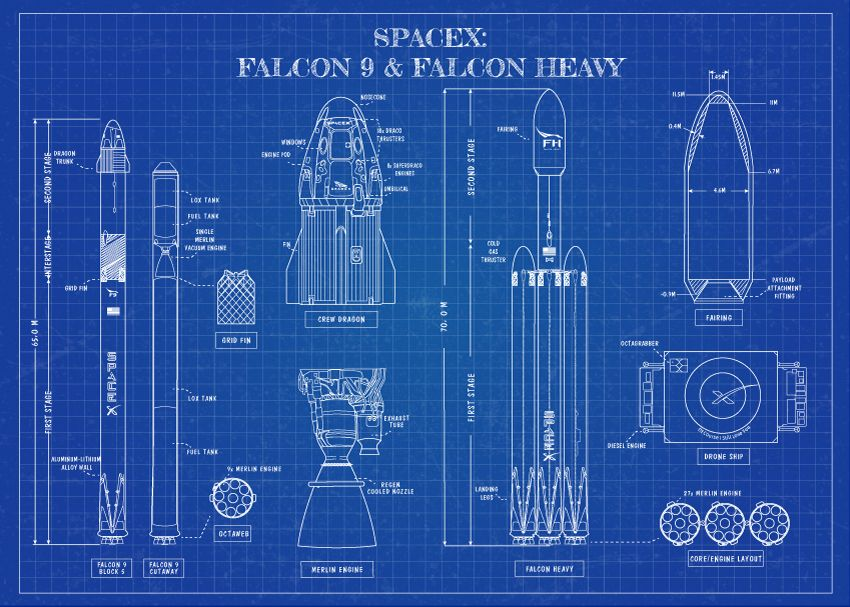
\includegraphics[width=0.4\textwidth]{gambar/cetakbiru.jpg}

  % Ubah sesuai dengan keterangan gambar yang diinginkan.
  \caption{Cetak biru roket yang akan diuji coba. \cite{cetakbiruspacex}}
  \label{fig:cetakbiru}
\end{figure}

\lipsum[9-11]

% Contoh pembuatan tabel.
\begin{table}
  \caption{Contoh tabel sederhana}
  \label{tab:tabelsederhana}
  \centering
  \begin{tabular}{lll}
    \toprule
    Heading1 & Heading2 & Heading3  \\
    \midrule
    One      & Two      & Three     \\
    Four     & Five     & Six       \\
    \bottomrule
  \end{tabular}
\end{table}

% Contoh pembuatan potongan kode.
\begin{lstlisting}[
  language=C++,
  caption={Program halo dunia.},
  label={lst:halodunia}
]
#include <iostream>

int main() {
    std::cout << "Halo Dunia!";
    return 0;
}
\end{lstlisting}

\lipsum[12]

% Contoh pembuatan daftar.
\begin{enumerate}
  \item \lipsum[13][1-4]
  \item \lipsum[13][5-8]
  \item \lipsum[13][9-12]
\end{enumerate}

\lipsum[14-15]

% Ubah judul dan label berikut sesuai dengan yang diinginkan.
\section{Hasil \& Pembahasan}
\label{sec:hasil}

% Ubah paragraf-paragraf pada bagian ini sesuai dengan yang diinginkan.

% Contoh input beberapa gambar pada halaman.
\begin{figure*}
  \centering
  \subfloat[Modul koneksi]{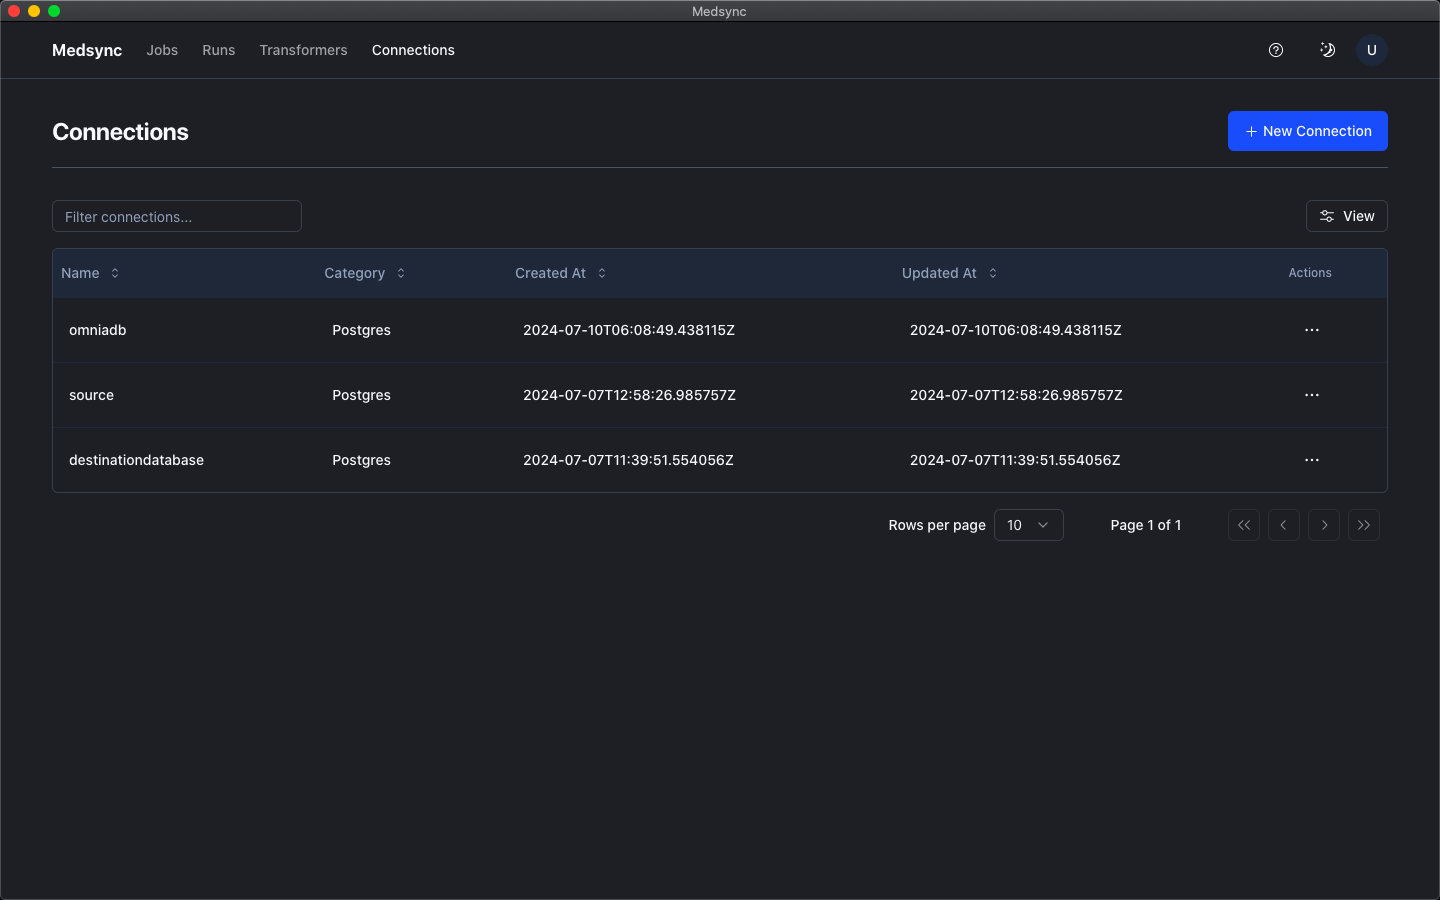
\includegraphics[width=.4\textwidth]{gambar/tampil-kon-bl.png}
    \label{fig:hasila}}
  \hfil
  \subfloat[Modul pekerjaan sinkronisasi]{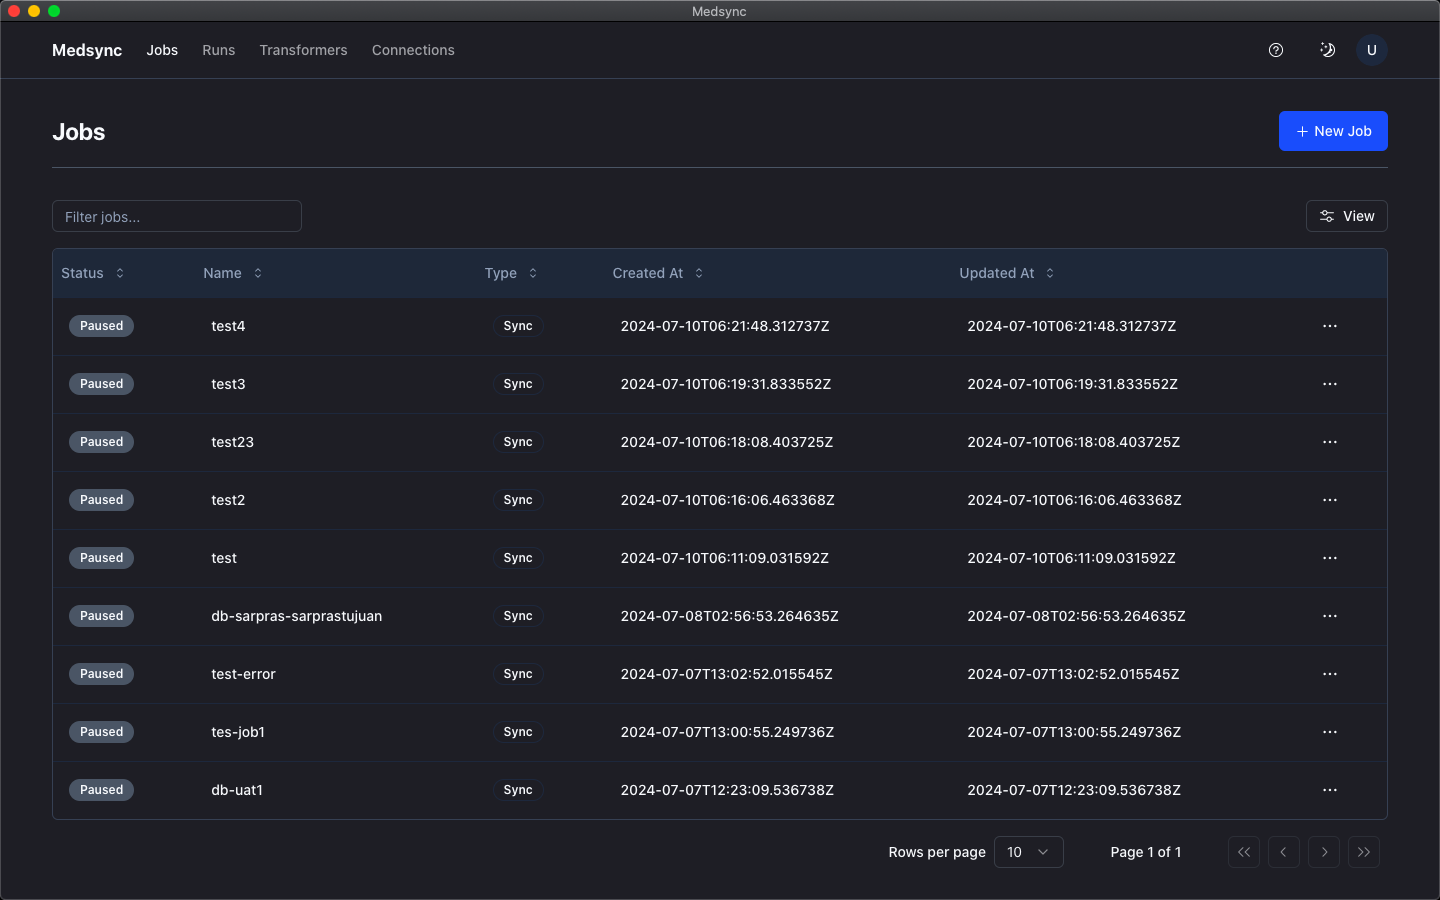
\includegraphics[width=.4\textwidth]{gambar/tampil-jon-bl.png}
    \label{fig:hasilb}}
  \hfil
  \subfloat[Modul eksekusi sinkronisasi]{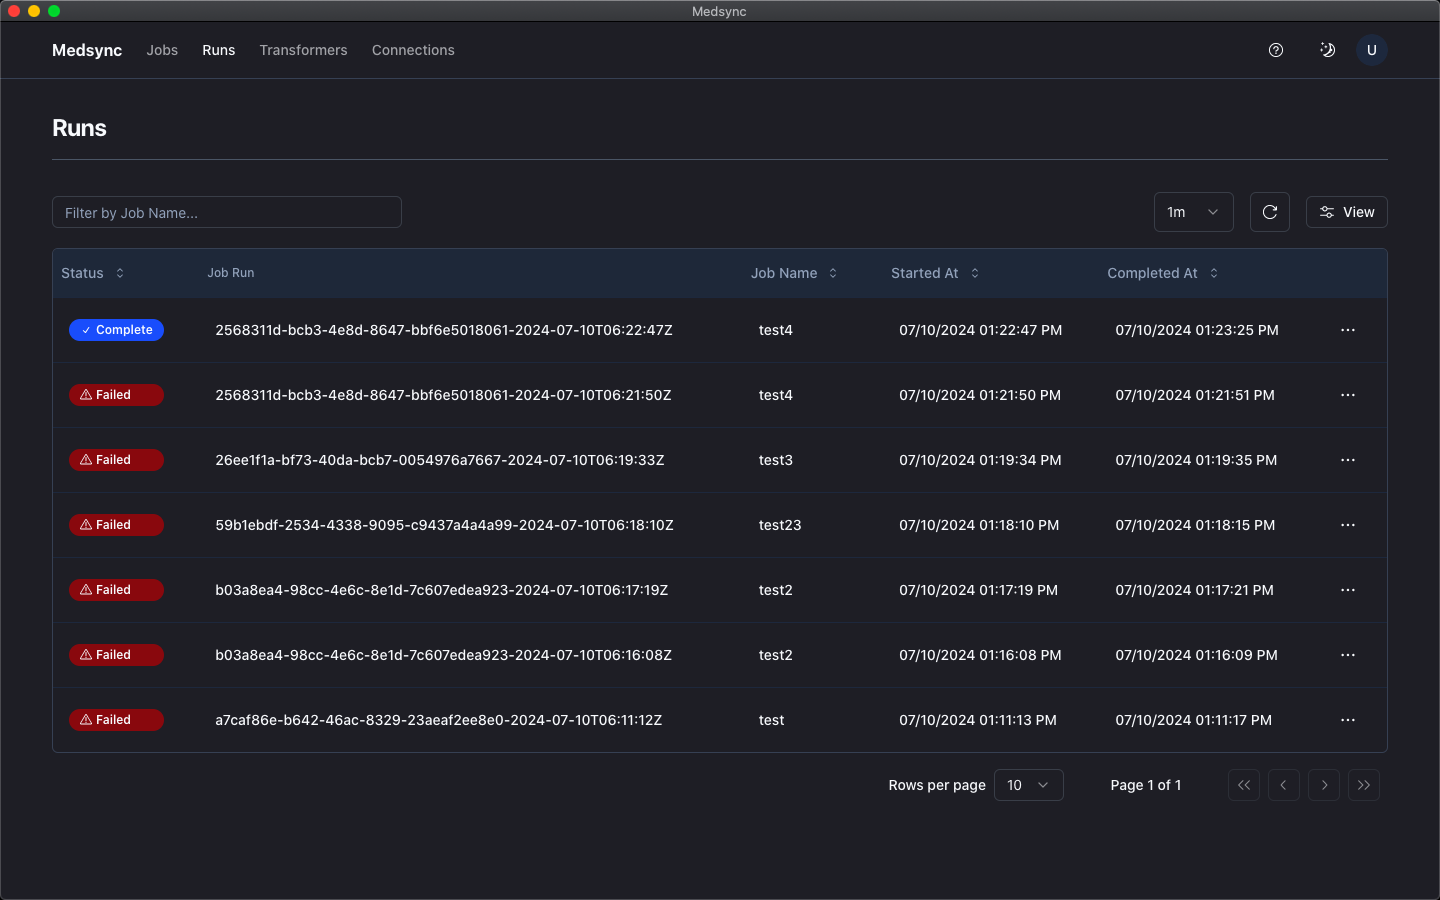
\includegraphics[width=.4\textwidth]{gambar/eksekuki-tampil-bl.png}
    \label{fig:hasilc}}
  \hfil
  \caption{Hasil Implementasi Perangkat Lunak}
  \label{fig:hasil}
\end{figure*}

\subsection{Implementasi}
Hasil implementasi Pada Gambar \ref{fig:hasil} menunjukkan tampilan pada tiga modul yang menjadi 
fondasi utama dalam menyelesaikan proses migrasi, yaitu modul koneksi, modul pekerjaan sinkronisasi, dan modul eksekusi sinkronisasi. Modul koneksi digunakan untuk menyimpan informasi koneksi basis data yang digunakan baik sebagai sumber ataupun tujuan pada proses sinkronisasi. Modul pekerjaan sinkronisasi digunakan untuk membuat proses sinkronisasi. Modul eksekusi digunakan untuk menampilkan setiap eksekusi yang dilkaukan pada pekerjaan sinkronisasi. 

\subsection{Pembahasan}
Implementasi aplikasi sesuai dengan \emph{use-case} memerlukan pengujian setelahnya guna memastikan seluruh fungsionalitas berjalan dengan semestinya. Pengujian dilakukan dengan membandingkan keluaran fungsi terkait \emph{use-case} dengan keluaran yang seharusnya dihasilkan oleh fungsi tersebut. Jika keduanya menghasilkan nilai yang sama, maka dapat disimpulkan bahwa fungsi yang mendukung \emph{use-case} tersebut telah berhasil. Selain pengujian pada fungsi, dilakukan juga pengujian terhadap tampilan aplikasi dengan melakukan debugging manual. Proses debugging manual ini bertujuan untuk memastikan bahwa antarmuka pengguna berfungsi sebagaimana mestinya, tampilan visualnya sesuai dengan desain yang diinginkan, serta interaksi pengguna berjalan tanpa hambatan. Pengujian frontend ini melibatkan identifikasi elemen antarmuka yang perlu diuji, pengembangan skenario pengujian untuk setiap elemen, dan pelaksanaan pengujian untuk memastikan bahwa semua elemen berfungsi dengan benar. Tabel \ref{tbl:fungsional} menyajikan hasil pengujian fungsionalitas.

\begin{table}
  \caption{Hasil pengujian fungsionalitas}
  \label{tab:fungsional}
  \centering
  \begin{tabular}{lll}
    \toprule
    \textbf{Kode} & \textbf{Nama Fitur} & \textbf{Hasil Uji} \\
    \midrule
    UC1-01 & Daftar & Berhasil \\
  UC1-02 & Masuk & Berhasil \\
%   \hline
 UC1-03 & Keluar & Berhasil \\
%   \hline
 UC2-01 & Tambah koneksi & Berhasil \\
%   \hline
 UC2-02 & Tampil semua koneksi & Berhasil \\
%   \hline
 UC2-03 & Tampil detail koneksi & Berhasil \\
%   \hline
UC2-04 & Ubah koneksi & Berhasil \\
%   \hline
 UC2-05 & Hapus koneksi & Berhasil \\
%   \hline
 UC2-06 & Test konfigurasi koneksi & Berhasil \\
%   \hline
 UC2-07 & Tampil informasi skema koneksi & Berhasil \\
%   \hline
 UC3-01 & Tambah pekerjaan sinkronisasi &  Berhasil\\
%   \hline
 UC3-02 & Tampil semua pekerjaan sinkronisasi & Berhasil \\
%   \hline
 UC3-03 & Tampil detail pekerjaan sinkronisasi & Berhasil \\
%   \hline
 UC3-04 & Hapus pekerjaan sinkronisasi & Berhasil \\
%   \hline
 UC3-05 & Jalan pekerjaan sinkronisasi & Berhasil \\
%   \hline
 UC3-06 & Tampil semua eksekusi sinkronisasi & Berhasil \\
%   \hline
 UC3-06 & Tampil detail eksekusi sinkronisasi & Berhasil \\
%   \hline
    \bottomrule
  \end{tabular}
\end{table}

Selanjutnya, dilakukan evaluasi dan pengujian terhadap kualitas data hasil migrasi. Evaluasi ini penting untuk memastikan bahwa data yang telah dipindahkan ke sistem baru tetap akurat, lengkap, dan konsisten. Proses evaluasi ini melibatkan beberapa tahapan, antara lain validasi data, verifikasi data, dan pengujian integritas data. Validasi data dilakukan untuk memastikan bahwa data yang dipindahkan sesuai dengan format dan standar yang ditetapkan. Verifikasi data bertujuan untuk mengecek kembali keakuratan data dengan membandingkannya dengan sumber data asli. Sementara itu, pengujian integritas data dilakukan untuk memastikan bahwa hubungan antar data tetap terjaga dengan baik dalam sistem baru.  
    
Untuk mendukung pengujian ini, penulis menyiapkan basis data sumber yang merupakan basis data PostgreSQL dengan nama \textbf{Sarpras} dan basis data tujuan yang merupakan basis data PostgreSQL dengan nama \textbf{SarprasTujuan}. Proses uji kualitas dilakukan dengan membandingkan jumlah baris pada basis data SarprasTujuan dengan basis data Sarpras. Langkah ini penting untuk memastikan bahwa seluruh data telah berhasil dipindahkan tanpa ada yang hilang atau terduplikasi. Selain membandingkan jumlah baris, proses uji kualitas juga melibatkan pemeriksaan beberapa aspek lain, seperti konsistensi data antar tabel dan validitas data individual. Pemeriksaan ini bertujuan untuk memastikan bahwa setiap entri data pada basis data tujuan sesuai dengan entri pada basis data sumber.\textbf{Tabel \ref{tab:baris}} merupakan hasil eksekusi query jumlah baris pada setiap tabel basis data Sarpras dan SarprasTujuan.

\begin{table}
  \caption{Hasil pengujian perbandingan jumlah baris}
  \label{tab:baris}
  \centering
  \begin{tabular}{lll}
    \toprule
    \textbf{Nama tabel} & \textbf{Sarpras} & \textbf{SarprasTujuan} \\
    \midrule
    migrations & 29 & 29 \\
    
    subunits & 17 & 17 \\
    
    users & 219 & 219 \\
    
    units & 3 & 3 \\
    
    subunit\_members & 121 & 121 \\
    
    squads & 6 & 6 \\
    
    members & 212 & 212 \\
    
    squad\_members & 76 & 76 \\
    
    instruments & 6 & 6 \\
    
    passcodes & 142 & 142 \\
    
    locations & 9 & 9 \\
    
    location\_units & 7 & 7 \\
    
    cars & 29 & 29 \\
    
    interval\_schedules & 10639 & 10639 \\
    
    shift\_schedules & 4 & 4 \\
    \bottomrule
  \end{tabular}
  \end{table}

    Berdasarkan hasil \ref{tab:baris}, ada beberapa hal yang perlu didiskusikan terkait dengan pengujian dan sinkronisasi data. Pertama, pengujian terkait uji kualitas data berhasil dibuktikan dengan jumlah tabel dan perbandingan antar jumlah baris di kedua basis data untuk masing-masing tabel yang memiliki nilai yang sama. Keberhasilan dalam uji kualitas data ini menunjukkan bahwa proses migrasi telah dilakukan dengan benar dan semua data telah terintegrasi dengan baik ke dalam sistem baru. Hal ini memberikan keyakinan bahwa data di basis data tujuan dapat digunakan untuk operasional sehari-hari tanpa masalah. Selain itu, kesamaan jumlah baris juga mengindikasikan bahwa tidak ada data yang hilang atau terduplikasi selama proses migrasi. Hal tersebut penting karena data yang hilang bisa menyebabkan kekurangan informasi yang diperlukan, sedangkan data yang terduplikasi bisa menyebabkan inkonsistensi dan kesalahan dalam analisis data.

    Langkah berikutnya setelah pengujian kualitas data migrasi adalah melakukan pengecekan konsistensi dan validitas data secara lebih mendalam. Pengecekan konsistensi ini penting untuk memastikan bahwa relasi antar tabel dalam basis data tetap utuh dan tidak mengalami anomali setelah proses migrasi. Selain itu, dilakukan pula uji lebih mendalam seperti pengujian nilai-nilai unik, pengecekan referensi silang antar entitas, dan tipe kolom pada setiap tabel. Untuk memenuhi kebutuhan pengujuan tersebut, digunakan alat \emph{PostgresCompare}. Berdasarkan hasil uji \emph{PostgresCompare}, didapatkan hasil bahwa terdapat 26 tabel pada kedua basis data identikal, mulai dari skema, nama tabel, tipe kolom pada setiap tabel, dan index pada setial tabel. 

    Namun demikian, dari pengujian sinkronisasi, penulis menemukan keterbatasan aplikasi. Salah satu masalah yang dihadapi adalah ketika dilakukan migrasi antara dua basis data yang memiliki tipe yang berbeda, seperti MySQL dan PostgreSQL. Permasalahan muncul karena perbedaan dalam pemetaan (mapping) antara struktur data PostgreSQL dan MySQL. Hal ini mempengaruhi proses sinkronisasi data yang seharusnya mulus, namun menjadi kompleks karena perbedaan dalam cara kedua sistem basis data ini memperlakukan beberapa tipe data dan indeks. Penulis berharap untuk penelitian selanjutnya, dapat dipertimbangkan untuk menerapkan pendekatan tipe basis data berbeda dalam konteks migrasi dan sinkronisasi. Pendekatan ini akan menguji kemampuan sistem untuk mentransfer data antara berbagai tipe basis data, seperti antara MySQL dan PostgreSQL, serta memperluas ruang lingkup adaptasi sistem terhadap perbedaan dalam struktur dan karakteristik tipe data yang digunakan oleh masing-masing sistem.

  

% \begin{longtable}{|l|l|l}
%   \caption{Hasil pengujian fungsionalitas} \label{tbl:fungsional} \\
%   \hline
%   \textbf{No.} & \textbf{Kode} & \textbf{Nama Fitur} & \textbf{Hasil Uji} \\
%   \hline
%   \endfirsthead
%   \endhead
%   \endfoot
  
%   \hline
%   \endlastfoot
  
%   1 & UC1-01 & Daftar & Berhasil \\
%   \hline
%   2 & UC1-02 & Masuk & Berhasil \\
%   \hline
%   3 & UC1-03 & Keluar & Berhasil \\
%   \hline
%   4 & UC2-01 & Tambah koneksi & Berhasil \\
%   \hline
%   5 & UC2-02 & Tampil semua koneksi & Berhasil \\
%   \hline
%   6 & UC2-03 & Tampil detail koneksi & Berhasil \\
%   \hline
%   7 & UC2-04 & Ubah koneksi & Berhasil \\
%   \hline
%   8 & UC2-05 & Hapus koneksi & Berhasil \\
%   \hline
%   9 & UC2-06 & Test konfigurasi koneksi & Berhasil \\
%   \hline
%   10 & UC2-07 & Tampil informasi skema koneksi & Berhasil \\
%   \hline
%   11 & UC3-01 & Tambah pekerjaan sinkronisasi &  Berhasil\\
%   \hline
%   12 & UC3-02 & Tampil semua pekerjaan sinkronisasi & Berhasil \\
%   \hline
%   13 & UC3-03 & Tampil detail pekerjaan sinkronisasi & Berhasil \\
%   \hline
%   14 & UC3-04 & Hapus pekerjaan sinkronisasi & Berhasil \\
%   \hline
%   15 & UC3-05 & Jalan pekerjaan sinkronisasi & Berhasil \\
%   \hline
%   16 & UC3-06 & Tampil semua eksekusi sinkronisasi & Berhasil \\
%   \hline
%   17 & UC3-06 & Tampil detail eksekusi sinkronisasi & Berhasil \\
%   \hline
%   \end{longtable}


\section{Kesimpulan}
\label{sec:kesimpulan}

\blindtext


% use section* for acknowledgment
\ifCLASSOPTIONcompsoc
  % The Computer Society usually uses the plural form
  \section*{Acknowledgments}
\else
  % regular IEEE prefers the singular form
  \section*{Acknowledgment}
\fi

This work received support from the \href{https://latextemplates.github.io/IEEE/}{IEEE LaTeX Template}.


In the bibliography, use \texttt{\textbackslash textsuperscript} for ``st'', ``nd'', \ldots:
E.g., \enquote{The 2\textsuperscript{nd} conference on examples}.
When you use \href{https://www.jabref.org}{JabRef}, you can use the clean up command to achieve that.
See \url{https://help.jabref.org/en/CleanupEntries} for an overview of the cleanup functionality.

% trigger a \newpage just before the given reference
% number - used to balance the columns on the last page
% adjust value as needed - may need to be readjusted if
% the document is modified later
%\IEEEtriggeratref{8}
% The "triggered" command can be changed if desired:
%\IEEEtriggercmd{\enlargethispage{-5in}}

% Enable to reduce spacing between bibitems (source: https://tex.stackexchange.com/a/25774)
% \def\IEEEbibitemsep{0pt plus .5pt}

\bibliographystyle{IEEEtranN} % IEEEtranN is the natbib compatible bst file
% argument is your BibTeX string definitions and bibliography database(s)
\bibliography{pustaka/pustaka.bib}

\ \\ % empty line after bibliogpraphy and that statement
All links were followed on April 18, 2018.

\balance

\end{document}
